\chapter{Einleitung}

Im folgenden Abschnitt werden die aus technischer Sicht relevanten Aspekte genauer analysiert. Zu Beginn wird das Aufgabenumfeld in einem weiteren Sinne betrachtet, und die Kernelemente der Applikation aufgezeigt. Danach wird auf die Analyse und die Realisierung eingegangen. Der Hauptteil richtet sich vor allem an Entwickler, die an der Weiterentwicklung des Produktes interessiert sind.

\section{Big Picture}

Zur Übersicht wird das Umfeld der Applikation in einem Big Picture zusammengefasst.
Die Darstellung wird in drei Abschnitte uterteilt. Im obersten Abschnitt befinden sich alle Geräte, welche Daten liefern. Diese sind alle Android Aufnahmesysteme, welche in dieser Arbeit umgesetzt werden, sowie der RadioTourSpeaker, welcher bereits vorhanden ist. \\
Im mittleren Teil befindet sich die Serverseite. Diese besteht aus einem TourLiveServer, welcher alle Renndaten sammelt und einem Devicemanagement Server, welcher die Einstellungen aller Aufnahmesysteme speichert und die Möglichkeit bietet, diese zu bearbeiten.\\
Der unterste Abschnitt zeigt Beispiele von Parteien, die mit den Daten beliefert werden. Dies kann die Webseite sein, die in dieser Arbeit umgesetzt wird, jedoch auch Drittanbieter, die Interesse an diesen Daten haben.

\begin{figure}[H]
	\caption{BigPicture}
	\centering
	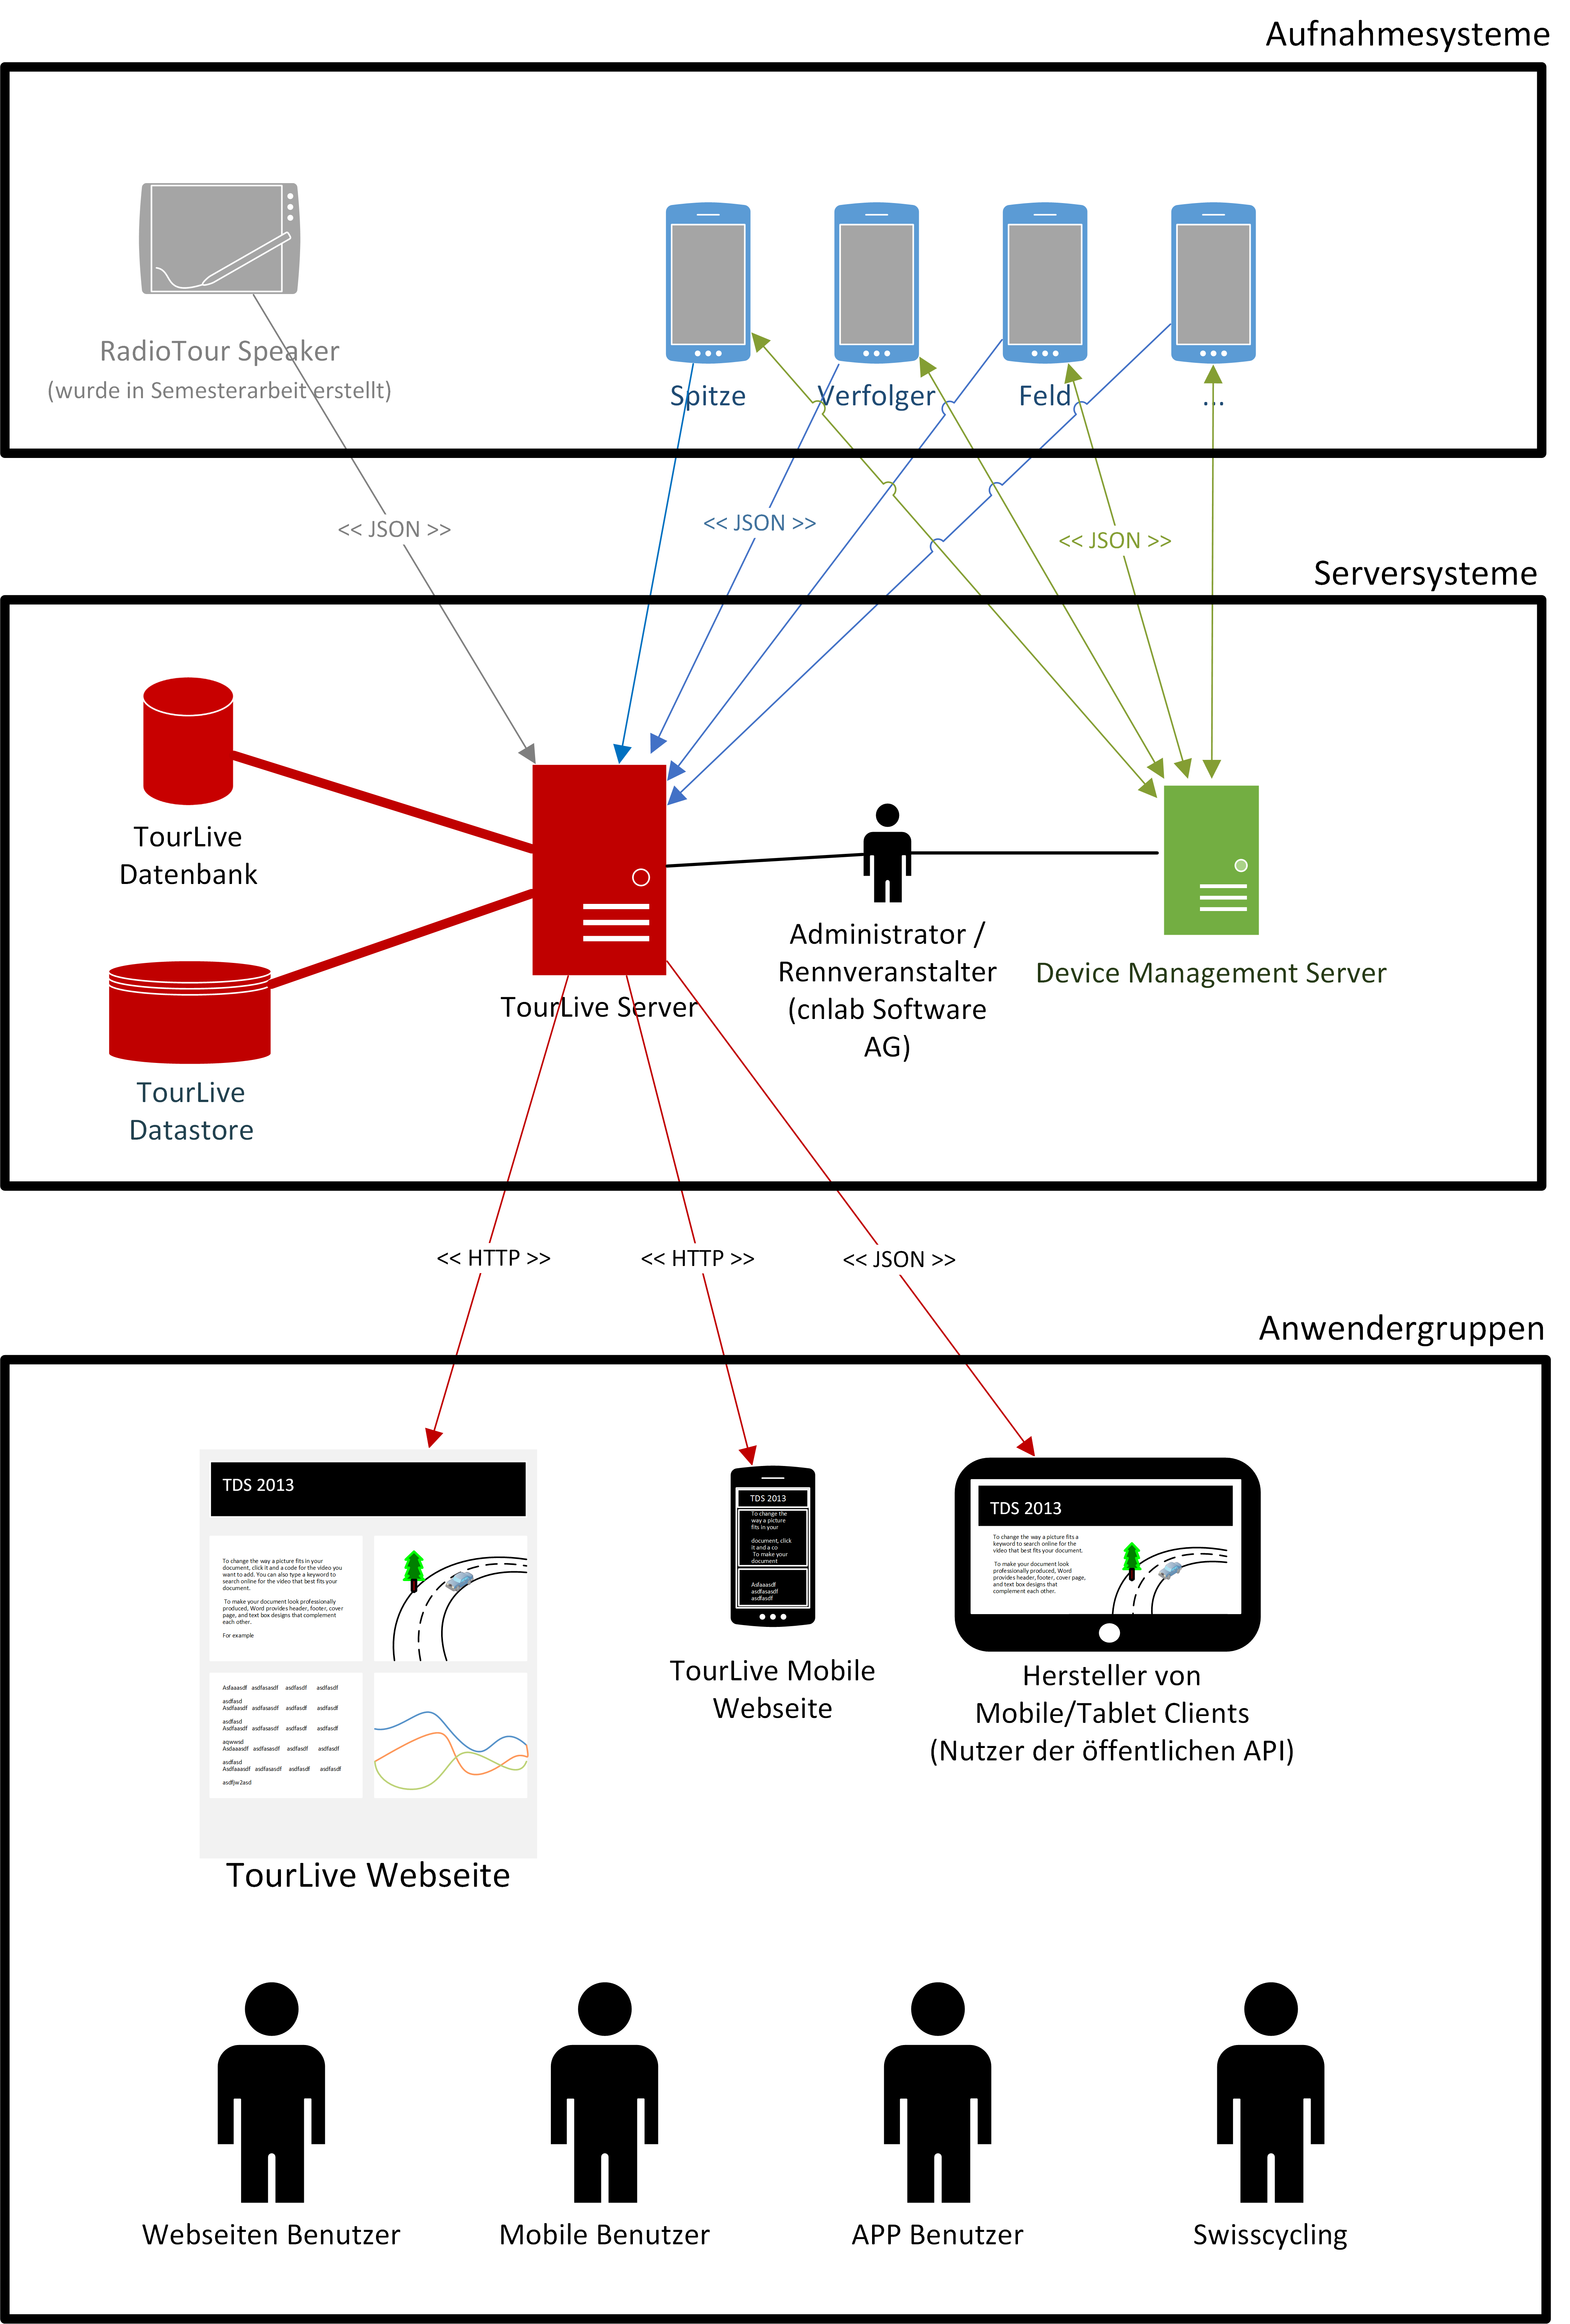
\includegraphics[height=200mm]{images/BigPicture.png}
\end{figure}

\section{Aufgabenteilung}

Hier kommt die Aufgabenteilung.